\chapter{Background}

\section{Representing Geometry}
\subsection{Triangles}
To develop an interactive 3D application, some kind of representation for the scene is needed. Traditionally, all geometric objects in a scene are represented by triangles. For example, to model a simple cube we can represent each of its faces using two triangles for a total of 12 triangles. The reason for using triangles is due to their geometric simplicity (triangles contain the fewest number of points that define a plane). Also, as dedicated Graphics Processing Units (GPUs) became more common they were designed with this traditional triangle rasterization in mind so they have specialized hardware to operate on triangles. In other words, triangles are fast to process.

But triangles do have some issues. Primarily, they do a good job of representing surfaces (since they are inherently 2D) but they don't lend themselves well to volumetric (3D) data. For example, a natural representation of a cloud would be a 3D volume filled with the density of the cloud at a given point within the volume. There are algorithms that can convert from a volumetric representation to a triangle one---marching cubes being the most popular---but it still only models an arbitrary isosurface as opposed to the actual volume.

\subsection{Voxels}
Voxels (volume elements) represent 3D objects in a natural way. A volumetric representation of an object is a 3D grid of cells (the voxels) which hold any data relevant to that voxel: color, transparency, and normal, to name a few. Recently, voxels have grown popular in the computer graphics field due to this natural representation of 3D objects. The main reason voxels were not used much in the past is due to the amount of memory required to store a voxelized representation as well as GPUs being specialized for triangle rasterization. This restriction has largely been lifted since modern GPUs have much more memory and general purpose GPU (GPGPU) computing has allowed programmers to work more easily with non-triangle based computing.

\begin{figure}[h]
\centering
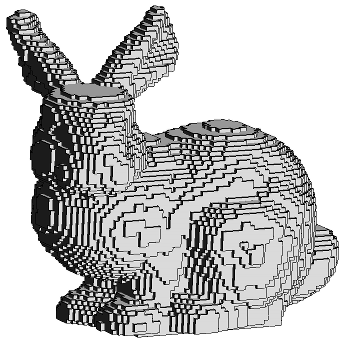
\includegraphics[scale=0.5]{bunny_voxel.png}
\caption{Voxelized representation of a bunny (image from \textit{http://cse.iitkgp.ac.in/\textasciitilde pb}).}
\label{fig:bunnyvoxel}
\end{figure}

\section{Radiance and the Rendering Equation}
In order to render a scene, we need some model of how light works. A physically accurate way to model light is with the concept of radiance. Radiance can be thought of as the radiant flux (the amount of light energy transferred per unit time) through some unit area. In other words, it is how much light is present at a given point and in which direction it is travelling. Spectral radiance is the same thing but incorporates the wavelength of the light as well. The rendering equation, which describes the radiance at a given point in space, was originally presented by Kajiya \cite{kajiya1986rendering}. The equation, with slightly more modern notation, is
\begin{equation*}
    L_o(\bm{x}, \omega_o, \lambda, t) = L_e(\bm{x}, \omega_o, \lambda, t) + \int_\Omega f_r(\bm{x}, \omega_i, \omega_o, \lambda, t)\ L_i(\bm{x}, \omega_i, \lambda, t)\ (\omega_i \cdot \bm{n})\ d\omega_i
\end{equation*}

where $\bm{x}$ is a point in space, $\omega_o$ is the direction of outgoing light, $\lambda$ is the wavelength of light, $t$ is time, $L_o$ is the total spectral radiance, $L_e$ is the emitted spectral radiance, $w_i$ is the direction of incoming light, $f_r$ is a bidirectional reflectance distribution function, $L_i$ is the incoming spectral radiance, $n$ is the surface normal at the point $\bm{x}$, and $\Omega$ is the unit hemisphere centered around $n$. Although it looks very complex, the result $L_o$ is essentially the light intensity at a given point when viewed from a particular angle, the term $L_e$ is the light emitted from the point towards the viewer, and the integral is calculating how much incoming light at a point is transferred towards the viewer. The dot product $(\omega_i \cdot \bm{n})$ attenuates the incoming light based on the angle between the incoming light and the normal.

\begin{figure}[h]
\centering
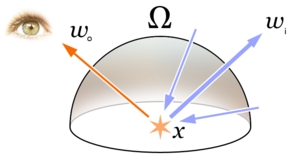
\includegraphics[scale=1.0]{rendering_eq.png}
\caption{Diagram representing the components of the rendering equation (image from \textit{https://en.wikipedia.org/wiki/Rendering\_equation}).}
\label{fig:renderingeq}
\end{figure}

Of course, in order to compute this we must at the very least discretize the problem. Furthermore, the complexity involved in calculating all of the integrals that would be needed to render a full scene as stated by the rendering equation is computationally infeasible. Thus we need some way to approximate this complete model of light.

\section{Global Illumination}
To approximate the rendering equation, first it is helpful to divide light into two categories: direct and indirect light. Direct light for a point is calculated by iterating through all light sources in a scene and computing their contribution to the point. This is relatively easy and straightforward. Indirect lighting for a point is the light accumulated from non-light sources in the scene, like the ambient light that is bounced off of other surfaces.

The term global illumination generally refers to a lighting model which attempts to accurately approximate indirect illumination. Approaches like having a constant ambient light amount and using ambient occlusion techniques like SSAO and HBAO do try to emulate some of the effects of indirect light but do not really attempt to accomplish full global illumination. For our algorithm, some of the main visual qualities we consider necessary are color bleeding, specular reflections, and limited light leaking (see Figure~\ref{fig:giqualities}). Here we give an overview of some techniques used to achieve more accurate global illumination.

\begin{figure}[h]
\centering
\makebox[\textwidth]{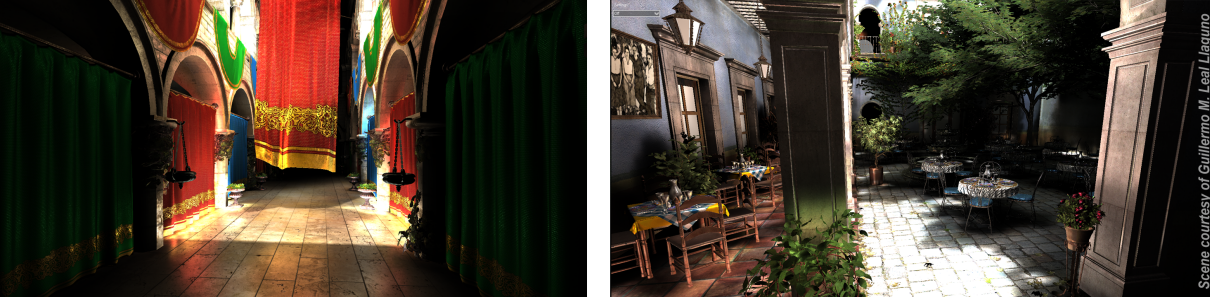
\includegraphics[width=\textwidth]{giqualities.png}}
\caption{Specular reflections can be seen on the ground of the left picture. Color bleeding can be seen on the archways of the left picture and on the column of the right picture. Images from~\cite{crassin2011interactive}.}
\label{fig:giqualities}
\end{figure}

\subsection{Monte Carlo Raytracing}
Raytracing is a common rendering technique which involves casting rays into a scene and determining color based on where the rays intersect. When a ray hits some geometry, direct lighting can be calculated by seeing if a ray from a light can `see' the intersection point. For indirect lighting, more work must be done. Monte Carlo Raytracing approximates the indirect light at a point by directly trying to approximate the surface integral over a hemisphere (as done in the rendering equation). This is done by only sending out a finite number of sampling rays to keep computation of the surface integral reasonable. The results, while impressive, still do not lend themselves well to real-time applications. Even with variations and improvements on the idea of raytracing, such as photon mapping, interactive frame rates are not achieved. 

\begin{figure}[h]
\centering
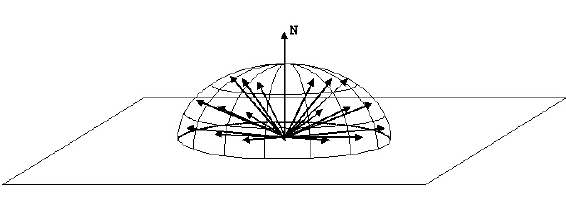
\includegraphics[scale=0.5]{sampling.png}
\caption{Sampling rays used to approximate an integral as would be done using Monte Carlo integration (image from \textit{https://computergraphics.stackexchange.com/questions/4979}).}
\label{fig:sampling}
\end{figure}

\subsection{Baked Lighting}
Another approach to global illumination is to approximate the radiance in a scene using some spatial representation. Then, when computing the lighting the radiance can be looked up and used to achieve global illumination. Baked lighting follows this approach by pre-processing a scene's geometry and light sources in order to compute the radiance in a scene. During run time, the radiance can be looked up quickly. The clear and major drawback of this method is it is completely static: if a light moves the radiance map created is no longer valid. Still, it is a great way to enhance visual quality when working with static lights.

\subsection{Voxel Cone Tracing}
The focus of much research, as well as this thesis, is on computing real-time global illumination with support for dynamic objects and lighting. Voxel cone tracing~\cite{crassin2011interactive} is relatively recent method for computing this that has gained some popularity, with variations being implemented by NVIDIA~\cite{nvidiavxgi} (which is incorporated into the Unreal Engine) and some games~\cite{mclaren2016cascaded}.

The general voxel cone tracing algorithm relies on approximating the scene's radiance using a voxelized spatial data structure, which then upscales (filters) the radiance in order to obtain adequate performance. To perform the actual lighting calculation, the radiance is sampled from the spatial data structure in such a way to minimize the amount of sampling without sacrificing quality. 


